% !TEX TS-program = pdflatex
% !TEX encoding = UTF-8 Unicode

% This is a simple template for a LaTeX document using the "article" class.
% See "book", "report", "letter" for other types of document.

\documentclass[11pt]{article} % use larger type; default would be 10pt

\usepackage[utf8]{inputenc} % set input encoding (not needed with XeLaTeX)
\usepackage[backend=biber, style=authoryear]{biblatex}
\addbibresource{bibliography.bib}
%%% Examples of Article customizations
% These packages are optional, depending whether you want the features they provide.
% See the LaTeX Companion or other references for full information.

%%% PAGE DIMENSIONS
\usepackage{geometry} % to change the page dimensions
\geometry{a4paper} % or letterpaper (US) or a5paper or....
% \geometry{margin=2in} % for example, change the margins to 2 inches all round
% \geometry{landscape} % set up the page for landscape
%   read geometry.pdf for detailed page layout information

%\usepackage{graphicx} % support the \includegraphics command and options

\usepackage[parfill]{parskip} % Activate to begin paragraphs with an empty line rather than an indent

%%% PACKAGES
\usepackage{booktabs} % for much better looking tables
\usepackage{array} % for better arrays (eg matrices) in maths
\usepackage{paralist} % very flexible & customisable lists (eg. enumerate/itemize, etc.)
\usepackage{verbatim} % adds environment for commenting out blocks of text & for better verbatim
\usepackage{subfig} % make it possible to include more than one captioned figure/table in a single float
\usepackage{graphicx}
\usepackage{csvsimple}
% These packages are all incorporated in the memoir class to one degree or another...

%%% HEADERS & FOOTERS
\usepackage{fancyhdr} % This should be set AFTER setting up the page geometry
\pagestyle{fancy} % options: empty , plain , fancy
\renewcommand{\headrulewidth}{0pt} % customise the layout...
\lhead{}\chead{}\rhead{}
\lfoot{}\cfoot{\thepage}\rfoot{}

%%% SECTION TITLE APPEARANCE
\usepackage{sectsty}
\allsectionsfont{\sffamily\mdseries\upshape} % (See the fntguide.pdf for font help)
% (This matches ConTeXt defaults)

%%% ToC (table of contents) APPEARANCE
\usepackage[nottoc,notlof,notlot]{tocbibind} % Put the bibliography in the ToC
\usepackage[titles,subfigure]{tocloft} % Alter the style of the Table of Contents
\renewcommand{\cftsecfont}{\rmfamily\mdseries\upshape}
\renewcommand{\cftsecpagefont}{\rmfamily\mdseries\upshape} % No bold!

%%% END Article customizations

%%% The "real" document content comes below...

\title{\vspace{-3.0cm}Urban Simulation Assessment}
%\date{} % Activate to display a given date or no date (if empty),
         % otherwise the current date is printed 

\begin{document}
\maketitle

%%%%%%%%%%%%%%%%%%%%%%%%%%%%%%%%%%%%%%%%%%%%%%%%%%%%%%%%%%%%%%%%%%%%%

\section{Part 1}

https://saintgimp.org/2013/01/22/merging-two-git-repositories-into-one-repository-without-losing-file-history/

\subsection{Introduction}

This is an analysis of resilience in the London tube network. The analysis uses a recursive function for node removal to calculate the marginal effect of a node's removal, pseudo-code for the function can be found in Appendix 1. Below, criteria for node removal and effect evaluation are discussed below. 


\subsection{Impact Evaluation}

Because the node removal criteria was decided in the context of the network effect metric, the network effect metric will be discussed first. 

\textbf{Calculate community metric for network to justify focus on distance?}
\textit{from igraph: cluster edge betweenness, cluster fast\_greedy, cluster\_label\_prop, cluster\_leading\_eigen, cluster louvain, cluster optimal, cluster spinglass, cluster walktrap.}

Because London's tube doesn't demonstrate strong sub clusters,breaking the network into isolates was investigated but not pursued. Instead, the focus will be on forcing tube users to travel further for longer on their journeys. 

This is investigated using shortest path and shortest topological path. Given the spatial nature of the london tubes, where edge attributes represent actual distances, true shortest path might be an attractive option. In the context of the London tube though, total time and effort are more important than total distance though. Trains can travel longer distances fairly rapidly while travelling through a high number of stations increases time dramatically because of the need to stop. Further, it is assumed that traveling through a higher number of stops implies a higher number of time and effort consuming train changes to switch. Thus by using geodesic, what is being maximized is the increase in stoppage time, and line change time for travelers in the network.

The statistics calculated to understand the effect of node removal include: \% of connected nodes in the graph, average of the node specific statistics above, 

The igraph package's mean\_distance\(\) function was used to compute the average shortest path between nodes in the network. The unconnected parameter was used to specify that nodes that were not connected to the largest cluster were counted as 1 + the longest possible geodesic, the actual longest geodesic is much less than this. This demonstrates the incompatibility of different network measures. There isn't really a way to compare the effect of a longer trip with the effect of removing a trip possibility entirely. To do that we would have to include alternate modes of transport like the bus network.  The actual longest geo

\subsection{Node Removal Criteria}

The function was run for measures that include, degree, betweeness, topological betweenness, closeness, topological closeness and eigenvector centrality. The correlations for these values across stations can be reviewed in figure 1. It was noted that correlations between weighted and topological measures were high, indicating that the distances between tube stations are fairly consistent so that the number of stations between two stations is a decent approximation of the distance. The correlation of measures betweenness and degree is also fairly high, indicating that tube stations at the middle of a line, with higher betweenness, also tend to have multiple lines, high degree. Correlations between eigenvector centrality and the other measures was very low, indicating that this does not give the same information as other metrics. Lastly, correlation between weighted and topological eigenvector centrality was 0 \textbf{indicating a problem with how they were calculated!}. 

In order to maximize the increase in travel time measured by the average length of geodesic paths, betweenness will be used to order node removals. This measure is the number of shortest paths between nodes that travel through a given node. Deleting the node with highest betweenness will force the highest number of trips to use an alternate, ostensibly longer, path through other stations. 

One note about this process, deleting nodes in some places creates isolates. In this investigation \textbf{this was not an issue I hope because for the first 10 or so nodes by betweenness, they were not the only node connecting any other node to the network.}

\begin{figure}
\centering
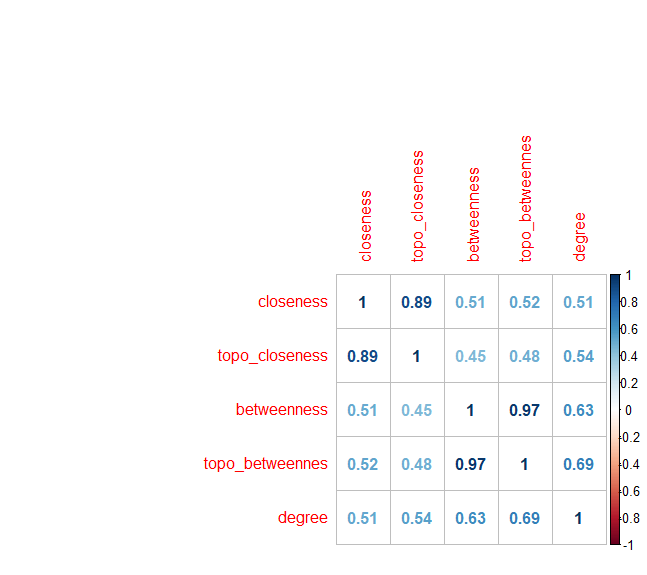
\includegraphics[width=0.8\textwidth]{Corr_tube_graph_node_stats}
\caption{Correlation between station/node metrics}
\end{figure}


\begin{center}
\csvautotabular{betfalse.csv}
\end{center}

% gotta reformat this probably asking about it on tex stack exchange

\begin{tabular}{|c|c|c|c|}\hline %
  \multicolumn{4}{|c|}{\bfseries Betweenness unconn is false}  \\ \hline
 & Node Deleted & Increase in Avg Geodesic & Components
  \csvreader[head to column names]{betfalse.csv}{} %
 {\\\index & \NodeDeleted & \IncreaseGeodesic & \Components} %
 \\\hline
 \end{tabular}
 


\begin{center}
\csvautotabular{bettrue.csv}
\end{center}

\begin{center}
\csvautotabular{eigtrue.csv}
\end{center}

\begin{center}
\csvautotabular{eigfalse.csv}
\end{center}




\subsection{Analysis}

When Kings Cross is deleted, it creates a new unconnected component out of the 11 stations on the north east end of the Picadilly line. In igraph, the two ways to handle this for the mean\_distance() function are either to exclude distances between those unconnected nodes and the rest of the network or to assume that the distance is one greater than the longest possible geodesic in the network, that is ,the number of nodes on the network. Data is included for both options. 

Looking at the effect data it seems reasonable to say that betweenness did a better job than eigenvector centrality of prioritizing nodes to remove. Using betweenness created more isolates. It's difficult to judge which method lengthened average shortest path the most because of the options for dealing with disconnected networks. This will be discussed in the conclusion. 



\subsection{Conclusions}

To improve this work, it would be good to add data about transportation networks besides the underground. In particular information about bus routes connected nodes would be useful because it would allow for a better estimate of average shortest path when subway stations become disconnected as the shortest path could then go through a bus route instead. Similarly, it would be good to include more granular data about where a rider would have to change trains. The current network assumes there's no cost to switch trains relative to staying on the same train passing through a station. Anyone who has walked from the Picadilly line to the Northern line at Kings Cross knows that there is a big difference. 

An improvement to the data would be to use travel time data instead of using distance as an approximation. 

Lastly, it would be interesting to build an igraph function that can compute average shortest path using edge weights since the current function cannot. This could confirm or reject the thought that tube stations are spaced fairly regularly based on the high correlation between weighted and topological centrality measures. 


%%%%%%%%%%%%%%%%%%%%%%%%%%%%%%%%%%%%%%%%%%%%%%%%%%%%%%%%%%%%%%%%%%%%%%%%%%%%%
\pagebreak

\section{Part 2}

\subsection{The Models}

\subsubsection{Unconstrained}

The model is constrained to the total flows of the system but flows out of an origin and into a destination can be any value between 0 and total system flows. 

This is useful for studying the change in connectivity between regions, for instance if a new transportation link was built. In particular, it is useful for studying long term effects of a change where residence and employment are more flexible. 

\subsubsection{Production }

The direction of flows can change but the total flows from each origin will remain constant. This is useful for studying the effect of a new employment or consumption location that changes the destinations of people going to work or to spend money. In terms of the matrix, it implies that the sums of the rows of the matrix are constant. 

\subsubsection{Attraction Constrained}

The source of flows into a region can change but the total flows into a region will remain constant. That is, any reduction in flows into a destination from another region will be fully replaced by flows into the destination from another region.  This could be used to study a new housing development that pulls people into residence in a different part of an area or a natural disaster that forces residents out of an area. Employers outside the area still need workers but will not be able to draw them from the same places after a housing change or natural disaster. In terms of the matrix the sums of the columns are held constant. 

\subsubsection{Doubly Constrained,}

Doubly constrained models could be used to test the short term effects of a change to transportation networks given that homes and businesses won't relocate but flexible behavior patterns like shopping could change almost immediately due to the change in accessibility or travel times between locations. In this model, the sums of both the columns and rows are held constant.


\textit{explain the role of the parameters}

\subsection{The Parameters}

Sensitivities to origin attributes, destination attributes, and linkage attributes

\subsection{A Scenario}

\textit{select a scenario and explore the consequences of varying model parameters and inputs on interaction flows and the origin/destination estimates}


What if Amazon built a big office in Long Island City? 



%%%%%%%%%%%%%%%%%%%%%%%%%%%%%%%%%%%%%%%%%%%%%%%%%%%%%%%%%%%%%%%%%%%%%%%%%%%%%

\section{Part 3}

\textit{define, compare and contrast Cellular Automata and Agent Based models}
Compare CA and ABM

While Cellular automata models are often viewed as separate modeling techniques, a more modern view of these methods considers them to be cousins or related in the sense that all CA are a subset of ABM. 

Expanding a CA model usually results in the creation of an ABM.  Cellular automata models are defined by a set of homogeneous cells that interact only with each other according to a defined set of input/output functions, e.g., if a cell with value 1 is surrounded by other cells f value 1 it's value becomes 0. The models can be extended to "n" states but all cells should be capable of reaching all n states to maintain the homogeneity of the cells. This can be contrasted with ABM where cells can have infinite heterogeneity and future states can be functions of the "environment" other cells or agents" and the cells own state. 

The simplicity of CA models make them very useful for studying mathematical processes whereas Agent Based Modeling flexibility make them useful for modeling more complex "real world" phenomena and make them more accessible to non-technical audiences. Often the value of ABM comes from the ability to conduct parameter sweeps, to study combination rules that apply to multiple conceptual processes with different parameter values. The value of cellular automata models tends to be focused on the effect of initialization states on the long term outcomes and equillibria of the model e.g. for the same model, outcomes are a function of the rule set and initialization values, where as agent based models tend to be calculated for a large number of initialization values in order to study the effect of model dynamics independent of initialization values that may not accurately reflect the real world. 

\textit{ vary model parameters to construct 3 scenarios, describe them, find time required to reach steady state, minimum runs required for statistically meaningful results. }


\subsection{Scenarios}

This will be an investigation of the behavior of an epidemic across different population types. The baseline population scenario will have mid-levels of immunity and recovery chances(50\%). The high immunity scenario will have immunity chance at 90\% and recovery chance at 10\% while the high recovery chance scenario will set recovery chance to 90\% and immunity chance to 10\%. 

\subsection{assumptions and preliminary investigation}

To understand a reasonable context for the scenarios above, behavior space was used to simulate a variety of initial-people and the number of people infected. 

\subsection{Questions}




Scenarios
\begin{itemize}
\item Baseline 
\item high immunity
\item high recovery
\end{itemize}

Record the run by using Behavior space ?
Change script so it infects people automatically?

How is this going to be 1000 words? 



\begin{verbatim}
use pseudocode
\end{verbatim}

XXXX words excluding headings, figures, and references. \\
\nocite{*}


\printbibliography


\end{document}
